
\chapter{Metodyka pracy oraz przygotowanie infrastruktury informatycznej}

\section{Wstęp}
Projekt powstawał w metodyce DevOps. Takie podejście pozwoliło na szybsze dostarczenie finalnego produktu. Wysoki poziom kooperacji wynikający z metodki DevOps pozwolił na zmniejszenie kosztów dostarczenia produktu oraz znaczne zwiększenie jego spójności. Potrzebna jest jednak mocno rozwinięta infrastruktura informatyczna służąca podtrzymaniu DevOps lifecycle.

\section{Pojęcia}
	\subsection{DevOps}
	DevOps~\cite{devops} to zestaw praktyk, narzędzi i filozofii kulturowej, które automatyzują i integrują procesy pomiędzy zespołami programistów oraz IT. Kładzie nacisk na wzmocnienie pozycji zespołu, komunikację i współpracę między zespołami oraz automatyzację technologii.
	Ruch DevOps rozpoczął się około 2007 roku, kiedy społeczności programistów i operatorów IT wyraziły zaniepokojenie tradycyjnym modelem rozwoju oprogramowania, w którym programiści piszący kod pracowali oddzielnie od operatorów, którzy wdrażali i wspierali kod. Termin DevOps, będący połączeniem słów \textit{development} i \textit{operations}, odzwierciedla proces integracji tych dyscyplin w jeden, ciągły proces.
\begin{figure}[H]
\centering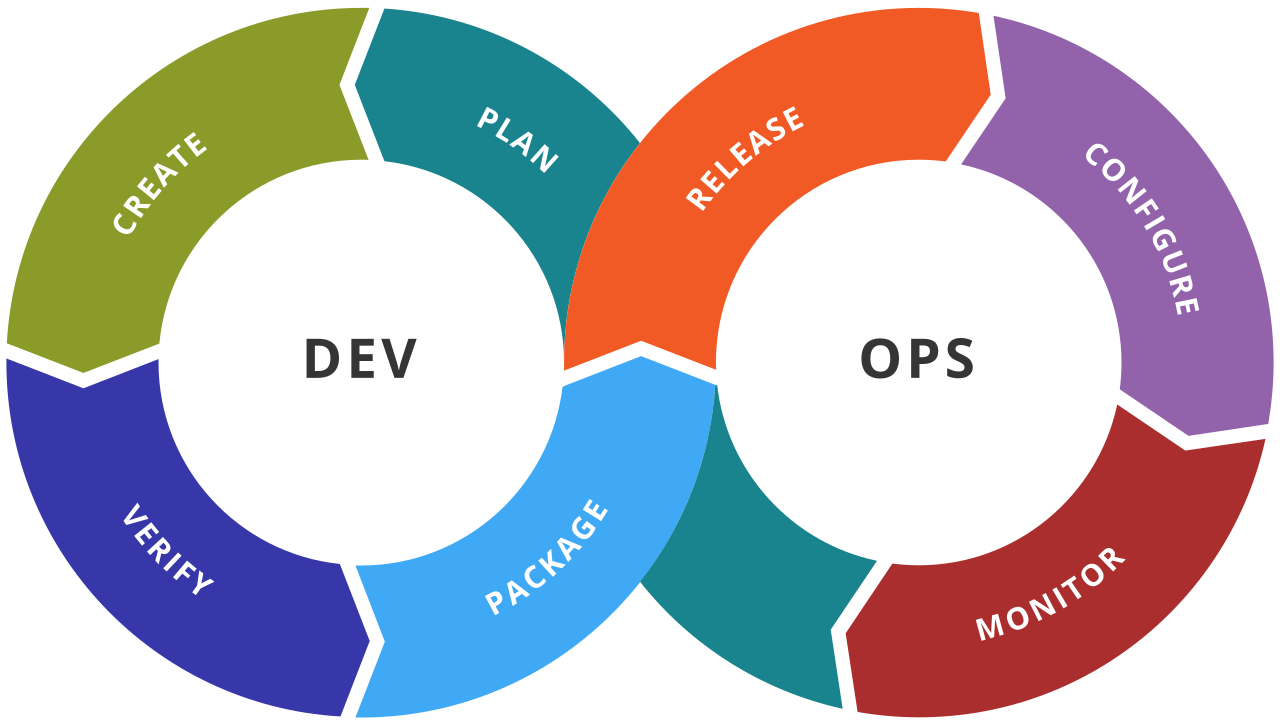
\includegraphics[width=10cm]{figures/devops_lifecycle}
\caption{Schemat DevOps lifecycle~\cite{devops_lifecycle}}\label{rys:DevOps lifecycle}
\end{figure}

	\subsection{Continous Integration and Continous Deployment}
	\textit{Continous Integration and Continous Deployment} (CI/CD)~\cite{ci} to metoda częstego dostarczania aplikacji do klientów poprzez wprowadzenie automatyzacji do etapów tworzenia aplikacji. Główne pojęcia przypisane do CI/CD to ciągła integracja, ciągłe dostarczanie i ciągłe wdrażanie. CI/CD jest rozwiązaniem problemów, jakie integracja nowego kodu może powodować dla zespołów programistycznych i operacyjnych.
	W szczególności, CI/CD wprowadza ciągłą automatyzację i ciągłe monitorowanie w całym cyklu życia aplikacji, od fazy integracji i testowania po dostarczanie i wdrażanie. Łącznie, te połączone praktyki są często określane jako CI/CD i są wspierane przez zespoły programistów i operatorów pracujących razem z podejściem DevOps lub SRE (\textit{site reliability engineering}).
	
	\subsection{Kontrola wersji}
	Kontrola wersji~\cite{version_control}, znana również jako kontrola źródła, jest praktyką śledzenia i zarządzania zmianami w kodzie oprogramowania. Systemy kontroli wersji to narzędzia programowe, które pomagają zespołom programistów zarządzać zmianami w kodzie źródłowym w czasie.


\section{Narzędzia i technologie}
	\subsection{Amazon Web Services}
	\textit{Amazon Web Services} (AWS)~\cite{aws} jest spółką zależną firmy Amazon, dostarczającą platformy chmury obliczeniowej na żądanie oraz interfejsy API osobom prywatnym, firmom i rządom na zasadzie \textit{pay-as-you-go}. Te usługi internetowe w chmurze obliczeniowej zapewniają różnorodne podstawowe abstrakcyjne elementy infrastruktury technicznej oraz narzędzia i bloki do obliczeń rozproszonych. Jedną z tych usług jest \textit{Amazon Elastic Compute Cloud} (EC2), która pozwala użytkownikom mieć do dyspozycji wirtualny klaster komputerów, dostępny przez cały czas, przez Internet. Wirtualne komputery AWS emulują większość atrybutów prawdziwego komputera, w tym sprzętowe jednostki centralne (CPU) i procesory graficzne (GPU) do przetwarzania danych, pamięć lokalną/RAM, pamięć masową HDD/SSD, wybór systemów operacyjnych, sieci oraz wstępnie załadowane oprogramowanie użytkowe, takie jak serwery internetowe, bazy danych i zarządzanie relacjami z klientami (CRM).
	
	\subsection{Git}
	Git~\cite{git} to darmowe narzędzie open-source służące do kontroli wersji, zaprojektowane do obsługi wszystkiego, od małych do bardzo dużych projektów z dużą prędkością i wydajnością.	
	
	\subsection{GitHub}
	GitHub~\cite{github} jest dostawcą hostingu internetowego dla rozwoju oprogramowania i kontroli wersji przy użyciu Git. Oferuje on funkcje rozproszonej kontroli wersji i zarządzania kodem źródłowym (SCM) Git, a także własne funkcje.
	
	\subsection{Docker}
	Docker~\cite{docker} to platforma konteneryzacji typu open source. Umożliwia ona programistom pakowanie aplikacji w kontenery - ustandaryzowane komponenty wykonywalne łączące kod źródłowy aplikacji z bibliotekami systemu operacyjnego (OS) i zależnościami wymaganymi do uruchomienia tego kodu w dowolnym środowisku. Kontenery upraszczają dostarczanie aplikacji rozproszonych i stają się coraz bardziej popularne w miarę jak organizacje przechodzą na rozwój cloud-native i hybrydowe środowiska wielochmurowe.
	
	\subsection{CircleCI}
	CircleCI~\cite{circleci} jest platformą obsługującą \textit{Continous Integration and Continous Delivery} (CICD), która pomaga zespołom programistycznym szybko i pewnie wypuszczać kod poprzez możliwość tworzenia \textit{pipeline} automatyzujących proces budowania, testowania i wdrażania. Pozwala to zespołom szybko się rozwijać, łatwo skalować i budować spójne produkty.
	\begin{itemize}
	\item \textit{Pipeline} jest jednostką pracy najwyższego poziomu, obejmującą cały plik ,,.circleci/config.yml'' projektu. Pipeline'y zawierają workflow'y, które koordynują zadania. Mają one ustalony, liniowy cykl życia i są powiązane z konkretnym aktorem. Pipeline'y uruchamiają się po wprowadzeniu zmiany do projektu, który zawiera plik konfiguracyjny CircleCI, a także mogą być zaplanowane, uruchamiane ręcznie za pomocą aplikacji CircleCI lub interfejsu API.
	\end{itemize}
\begin{figure}[H]
\centering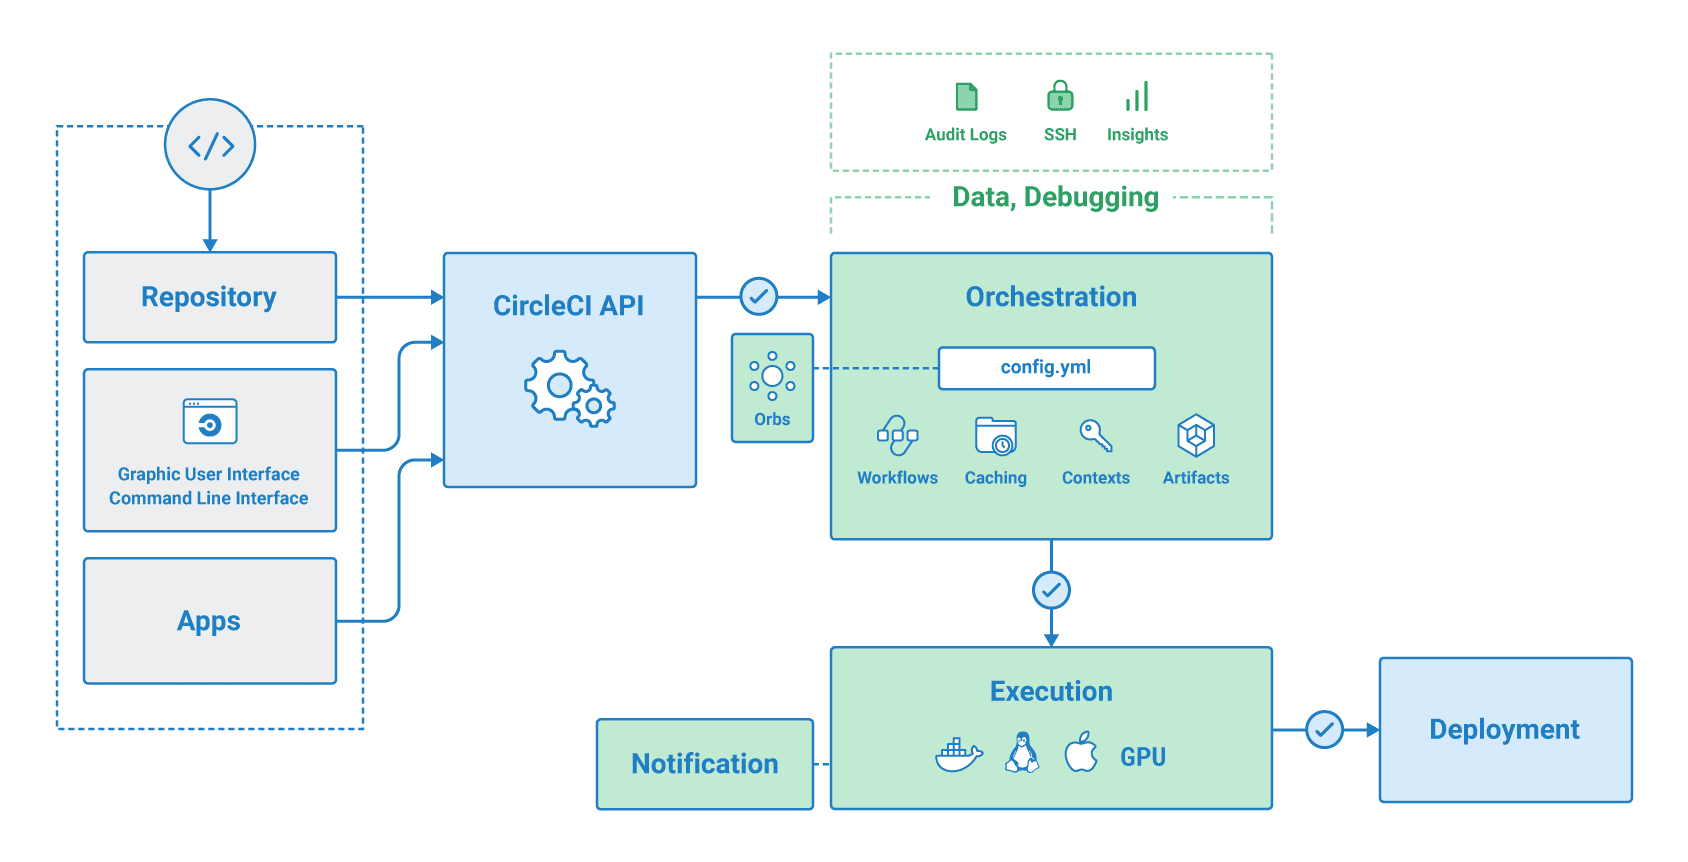
\includegraphics[width=\textwidth]{figures/circleci_schema}
\caption{Diagram przedstawiający działanie CircleCI~\cite{circleci_schema}}\label{rys:CircleCI diagram}
\end{figure}

	\subsection{Secure Shell}
	\textit{Secure Shell} (SSH)~\cite{ssh} to protokół zdalnej administracji, który pozwala użytkownikom kontrolować i modyfikować zdalne serwery przez Internet. Usługa ta została stworzona jako bezpieczny zamiennik dla nieszyfrowanego protokołu Telnet i wykorzystuje techniki kryptograficzne, aby zapewnić szyfrowaną komunikację ze zdalnym serwerem. Zapewnia mechanizm uwierzytelniania zdalnego użytkownika, przesyłania danych wejściowych od klienta do hosta i przekazywania danych wyjściowych z powrotem do klienta.
	
	\subsection{tmux}
	tmux~\cite{tmux} jest multiplekserem terminali. Umożliwia tworzenie, dostęp i sterowanie wieloma terminalami z jednego ekranu. tmux może zostać odłączony od ekranu i kontynuować pracę w tle, a następnie ponownie dołączony.

\section{Przygotowanie infrastruktury informatycznej}
	\subsection{Przygotowanie strony serwerowej przy pomocy platformy AWS}
	Do przygotowania strony serwerowej aplikacji wykorzystano jedną z usług platformy \textit{Amazon Web Services} jaką jest \textit{Amazon Elastic Compute Cloud} (EC2). Do przygotowania serwera strony Frontend'owej oraz Backend'owej przygotowano dwie niezależne instancje usługi EC2. Obie z przygotowanych instancji są typu \textit{t2.micro} zawierającego się w ramach pakietu \textit{AWS Free Tier}. Dzięki wyborowi tego typu instancji udało się zachować zerowy wkład pieniężny na potrzeby pracy inżynierskiej. Zasoby możliwe do wykorzystania w ramach typu \textit{t2.micro} nie są wystarczające na przypadek skomercjalizowania projektu jednak w zupełności wystarczają na potrzeby przygotowania projektu w ramach pracy inżynierskiej.
System operacyjny wykorzystany na obu instancjach EC2 to \textit{Linux Ubuntu 20.04.3 LTS} w wersji serwerowej. Zastosowanie takiej wersji systemu zmniejsza zapotrzebowanie systemu na zasoby obliczeniowe przez ograniczenie procesów systemowych (np. brak GUI) dzięki czemu większa ilość zasobów może zostać udostępniona na potrzeby zadań serwerowych. W celu zwiększenia bezpieczeństwa komunikacji, \textit{Inbound Rules} oraz \textit{Outbound Rules} zostały skonfiguorwane tak aby jak najbardziej uszczegółowić typy możliwych połączeń z instancjami.
	
	\subsection{Przygotowanie CI/CD Pipeline przy pomocy platformy CircleCI}
	Do przygotowania CI/CD Pipeline wykorzystano platformę CircleCI. Cały proces przygotowano w taki sposób aby pipeline uruchamiany został w momencie wprowadzenia zmian w repozytorium. Job build'u i testowania uruchamiany jest dla każdych zmian wprowadzonych w zdalnym repozytorium. Job deployment'u uruchamiany jest tylko i wyłącznie, jeśli zmiany zostały wprowadzone w ramach branch'y \textit{main} oraz jeśli job build'u i testowania zakończył się bez błędów.
	
\begin{figure}[H]
\centering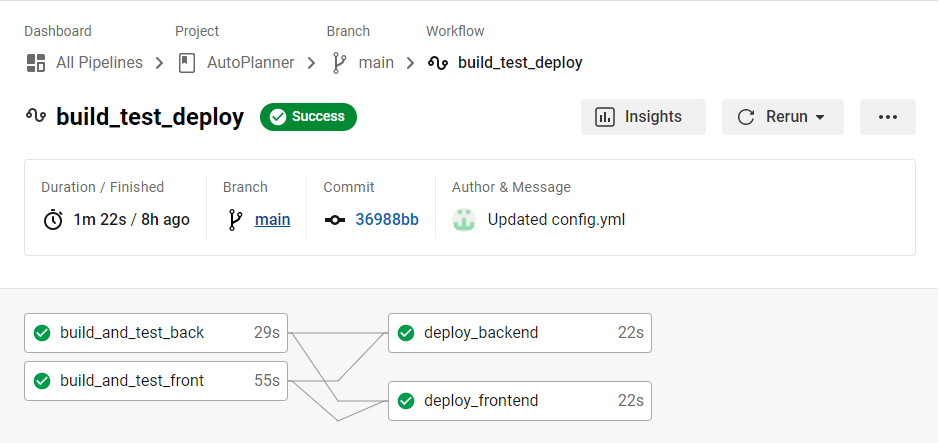
\includegraphics[width=\textwidth]{figures/ppl_flow}
\caption{Pipeline uruchomiony dla zmian wprowadzonych w branch'y \textit{main}.}
\end{figure}

\begin{figure}[H]
\centering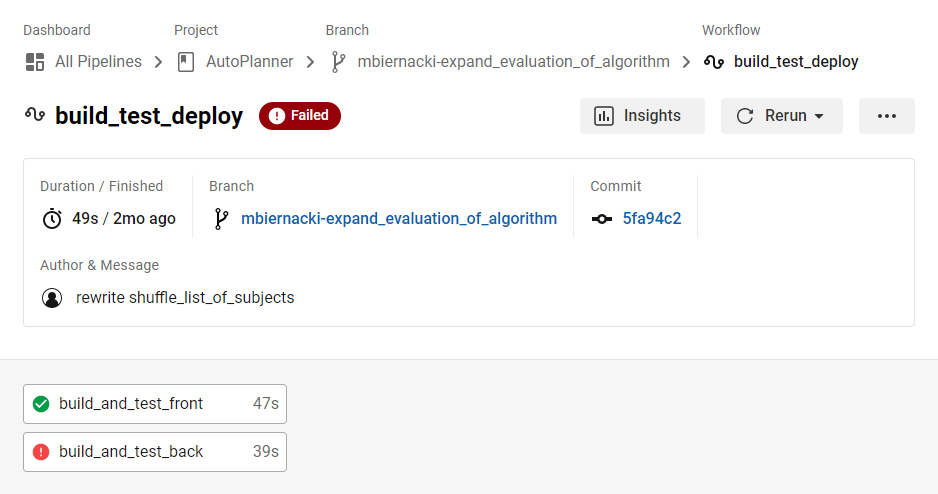
\includegraphics[width=\textwidth]{figures/ppl_flow_fail}
\caption{Pipeline, w którym wystąpiły błędy. Uruchomiony dla zmian wprowadzonych w branch'y innej niż \textit{main}.}
\end{figure}

	Każdy workflow składa się z zadań, na które składają się jeszcze mniejsze kroki podczas, których wywoływane mogą być polecenia shell'owe wykonywane w kontenerach Docker'owych stworzonych na potrzeby wykonania danego zadania. Platforma CircleCI umożliwia tworzenie własnych obrazów Docker'owych jak i zarówno dostarcza szereg gotowych rozwiązań przygotowanych w celu ułatwienia i przyśpieszenia tworzenia pipeline'y na potrzeby małych projektów. Na potrzeby projektu inżynierskiego utworzono workflow \textit{build\_test\_deploy} składający się z 4 zadań \textit{build\_and\_test\_back, build\_and\_test\_front, deploy\_frontend} oraz \textit{deploy\_backend}. (zob. listing 4.1) 
\begin{lstlisting}[caption=Część skryptu config.yml odpowiedzialna za określenie przebiegu workflow'u.]
workflows:
  build_test_deploy:
    jobs:
      - build_and_test_back
      - build_and_test_front
      - deploy_frontend:
          requires:
            - build_and_test_back
            - build_and_test_front
          filters:
            branches:
              only:
                - main
      - deploy_backend:
          requires:
            - build_and_test_back
            - build_and_test_front
          filters:
            branches:
              only:
                - main
\end{lstlisting} 

\begin{itemize}
\newpage
	\item \textit{build\_and\_test\_back} - podczas tego kroku budowany jest kontener Docker'owy na bazie obrazu z przygotowanym Pythonem w wersji 3.9. Na początku tego zadania w obrębie kontenera wykonywany jest checkout na branch, której zmiany wywołały start pipeline'y. Następnie wykonywany jest krok instalujący requirement'y projektu z pliku \textit{requirements.txt}. Kolejnym krokiem jest sformatowanie plików \textit{.py} przy pomocy gotowego rozwiązania jakim jest narzędzie Black. Następny krok to sprawdzenie kodu przy pomocy lintera \textit{pylint}. Wykorzystanie tego narzędzia zwiększa jakość publikowanego kodu oraz go standaryzuje w przypadku rozwijania oprogramowania przez wiele osób. Dwa ostatnie kroki odpowiedzialne są za uruchomienie testów jednostkowych backend'u oraz algorytmu. (zob. listing 4.2 oraz rys. 4.5)
	
\begin{lstlisting}[caption=Część skryptu config.yml odpowiadająca za wykonanie zadania \textit{build\_and\_test\_back}.]
build_and_test_back:
    docker:
      - image: cimg/python:3.9
    steps:
      - checkout
      - run:
          name: Install requirements
          command:
            sudo apt-get update;
            pip install --upgrade pip && pip install -r requirements.txt && pip install pylint
      - run:
          name: Format .py files
          command:
            pip install black && black $(git ls-files '*.py')
      - run:
          name: pylint
          command:
            pylint $(git ls-files '*.py')
      - run:
          name: unit_test_django
          command:
            cd Backend && python manage.py test backend_api
      - run:
          name: unit_test_algorithm
          command:
            cd Algorithm && pytest
\end{lstlisting} 
\newpage
\begin{figure}[H]
\centering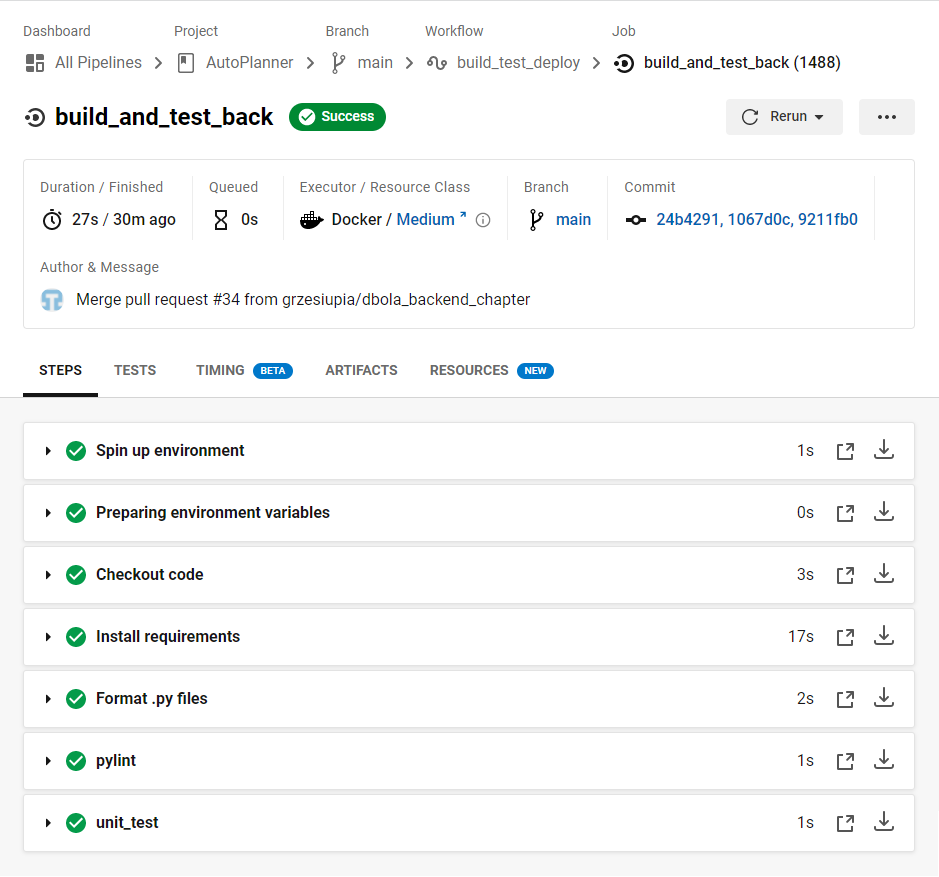
\includegraphics[width=\textwidth]{figures/circleci_test_back}
\caption{Przykładowy przebieg zadania \textit{build\_and\_text\_back}. Uruchomiony dla zmian wprowadzonych w branch'y \textit{main}.}
\end{figure} 

\newpage
	\item \textit{build\_and\_test\_front} - w tym zadaniu na początku budowany jest kontener dockerowy na bazie obrazu z przygotowanym Node.js w wersji 17.2.0. Następnie wykonywany jest checkout do branch'y, której zmiany wywołały start pipeline'y.  Kolejne dwa kroki odpowiedzialne są za przygotowanie środowiska tj. zaktualizowanie wersji Node.js do \textit{latest} oraz zainstalowanie dependencji projektu. W tak przygotowanym środowisku ostatnim krokiem jest uruchomienie testów jednostkowych z przygotowanego pliku (zob. Rozdział 8 - Testowanie). (zob. listing 4.3 oraz rys. 4.6)
\begin{lstlisting}[caption=Część skryptu config.yml odpowiadająca za wykonanie zadania \textit{build\_and\_test\_front}.]
build_and_test_front:
    docker:
      - image: cimg/node:17.2.0
    steps:
      - checkout
      - run:  
          name: Update node.js
          command:
            npm install node.js@latest
      - run:
          name: Install dependencies
          command:
            npm install ./Frontend
      - run:
          name: unit_tests
          command:
            cd Frontend &&
            npm run test:unit
\end{lstlisting}
\newpage
\begin{figure}[H]
\centering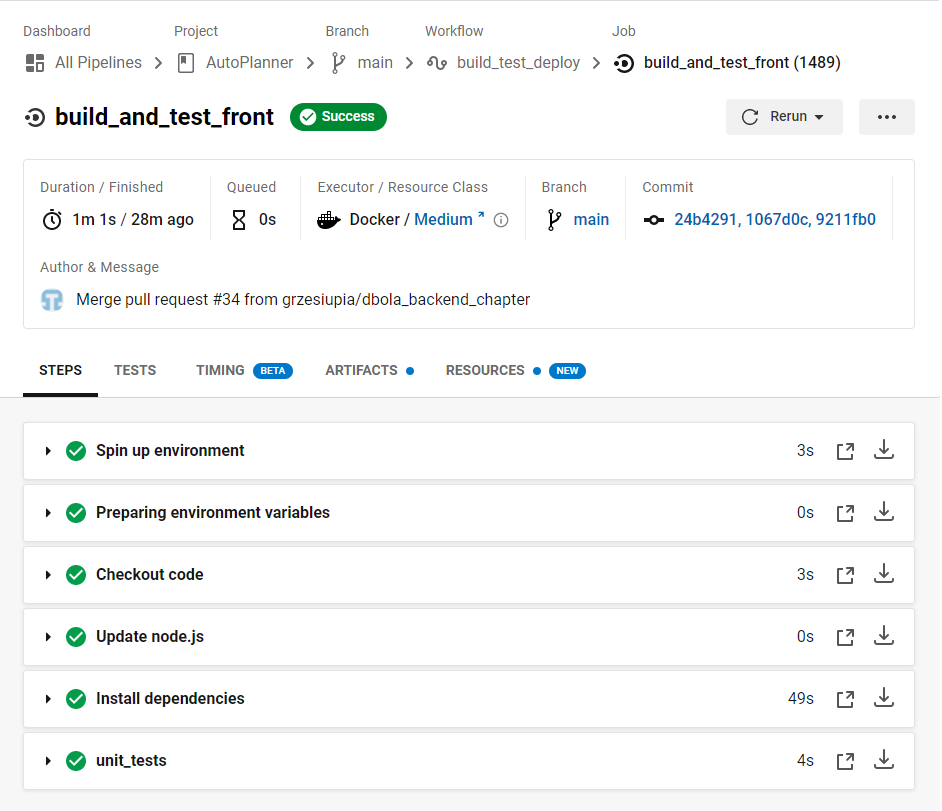
\includegraphics[width=\textwidth]{figures/circleci_test_front}
\caption{Przykładowy przebieg zadania \textit{build\_and\_text\_front}. Uruchomiony dla zmian wprowadzonych w branch'y \textit{main}.}
\end{figure}

\newpage
	\item \textit{deploy\_frontend} - w tym zadaniu głównym narzędziem jest aws-cli (\textit{AWS command line interface}). Pozwala on na obsługę instancji EC2 z poziomu shell'a. Pierwszym krokiem zadania jest checkout do branch'y, której zmiany wywołały wystartowanie pipeline'y. W nastepnym kroku ustawiany jest \textit{access\_key\_id} oraz \textit{secret\_access\_key} potrzebny do połączenia ssh. Dzięki wykorzystaniu zmiennych środowiskowych platformy CircleCI wartości te pozostają ukryte dla osób nie mających dostępu do projektu z poziomu platformy. Ostatnim jednak bardzo rozbudowanym krokiem jest połączenie z użyciem protokołu \textit{SSH} i wykonanie operacji deployment'u z poziomu instancji serwera. Po podłączeniu się do maszyny zdalnej wykonywane są takie czynności jak pull najnowszych zmian ze zdalnego repozytorium, reinstalacja dependencji oraz restart serwera frontend'owego. Po stronie serwera wykorzystywany jest terminal multiplexer \textit{tmux}. Dzięki otwarciu sesji w tle, jest możliwe wykonywanie innych czynności z równolegle działającym serwerem oraz utrzymanie sesji po zakończeniu sesji \textit{SSH}. (zob. listing 4.4 oraz rys. 4.7)
\begin{lstlisting}[caption=Część skryptu config.yml odpowiadająca za wykonanie zadania \textit{deploy\_frontend}.]
deploy_frontend:
    executor: aws-cli/default
    steps:
      - checkout
      - aws-cli/setup:
          aws-access-key-id: AWS_ACCESS_KEY_ID_FRONT
          aws-secret-access-key: AWS_SECRET_ACCESS_KEY_FRONT
      - run:
          name: deploy_frontend
          command: |
            sudo apt-get update

            # SSH to the server to deploy and Perform steps to deploy
            ssh -o StrictHostKeyChecking=no $EC2_USERNAME@$EC2_PUBLIC_DNS_FRONT 'cd GroupProject; 
            git pull --rebase;
            cd Frontend;
            npm install;
            tmux kill-session -t FRONTEND_SERVER
            sleep 5;
            tmux new-session -d -s "FRONTEND_SERVER";
            tmux send-keys -t FRONTEND_SERVER "npm run serve" C-m;
            exit'

            echo DONE! Successfully deployed to Frontend EC2 server.
\end{lstlisting}
\newpage
\begin{figure}[H]
\centering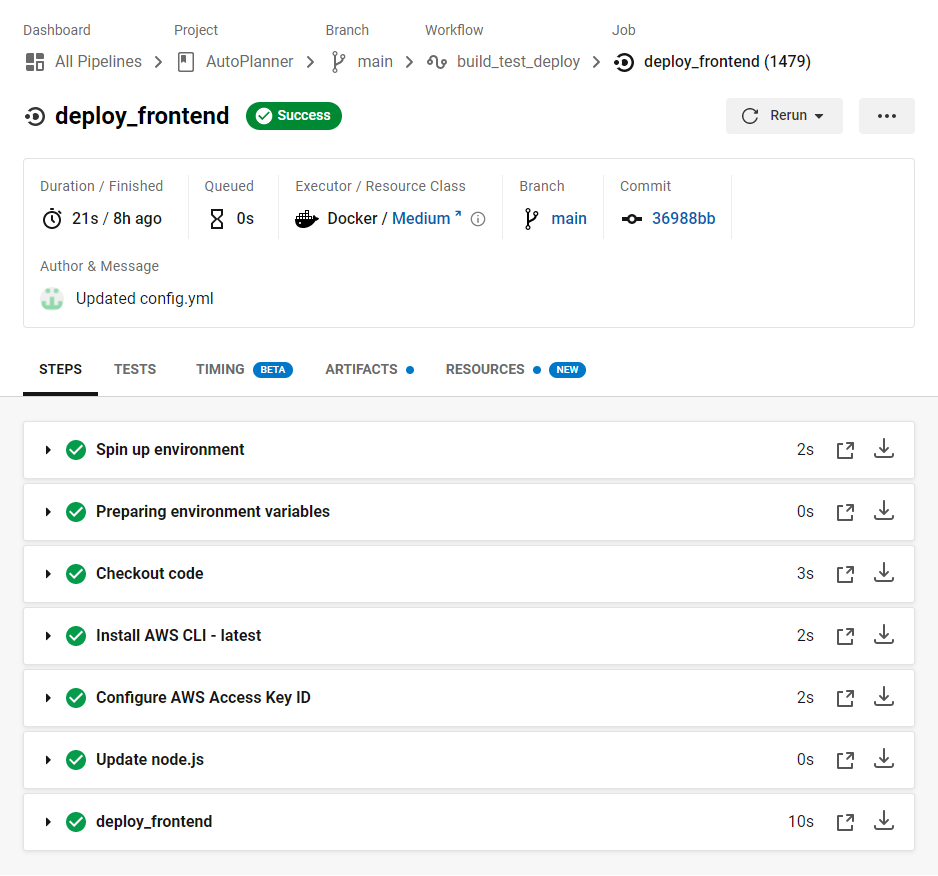
\includegraphics[width=\textwidth]{figures/circleci_deploy_front}
\caption{Przykładowy przebieg zadania \textit{deploy\_frontend}. Uruchomiony dla zmian wprowadzonych w branch'y \textit{main}.}
\end{figure}
	
\newpage
	\item \textit{deploy\_backend} - podobnie jak w zadaniu \textit{deploy\_frontend} głównym narzędziem jest aws-cli. Pierwszym krokiem zadania jest checkout do branch'y, której zmiany wywołały wystartowanie pipeline'y. W nastepnym kroku ustawiany jest \textit{access\_key\_id} oraz \textit{secret\_access\_key} potrzebny do połączenia ssh. Dzięki wykorzystaniu zmiennych środowiskowych platformy CircleCI wartości te pozostają ukryte dla osób nie mających dostępu do projektu z poziomu platformy. Ostatnim jednak bardzo rozbudowanym krokiem jest połączenie z użyciem protokołu \textit{SSH} i wykonanie operacji deployment'u z poziomu instancji serwera. Po podłączeniu się do maszyny zdalnej wykonywane są takie czynności jak pull najnowszych zmian ze zdalnego repozytorium, reinstalacja requirement'ów oraz restart serwera backend'owego. Po stronie serwera wykorzystywany jest terminal multiplexer \textit{tmux}. (zob. listing 4.5 oraz rys. 4.8)
\begin{lstlisting}[caption=Część skryptu config.yml odpowiadająca za wykonanie zadania \textit{deploy\_backend}.]
deploy_backend:
    executor: aws-cli/default
    steps:
      - checkout
      - aws-cli/setup:
          aws-access-key-id: AWS_ACCESS_KEY_ID_BACK
          aws-secret-access-key: AWS_SECRET_ACCESS_KEY_BACK
      - run:
          name: deploy_back
          command: |
            sudo apt-get update
            
            # SSH to the server to deploy and Perform steps to deploy
            ssh -o StrictHostKeyChecking=no $EC2_USERNAME@$EC2_PUBLIC_DNS_BACK 'cd GroupProject; 
            git pull --rebase;
            python -m pip install -r requirements.txt;
            cd Backend;
            tmux kill-session -t BACKEND_SERVER
            sleep 5;
            tmux new-session -d -s "BACKEND_SERVER";
            tmux send-keys -t BACKEND_SERVER "python3 manage.py runserver 0.0.0.0:8000" C-m;
            exit'

            echo DONE! Successfully deployed to Backend EC2 server.    
\end{lstlisting}
\newpage
\begin{figure}[H]
\centering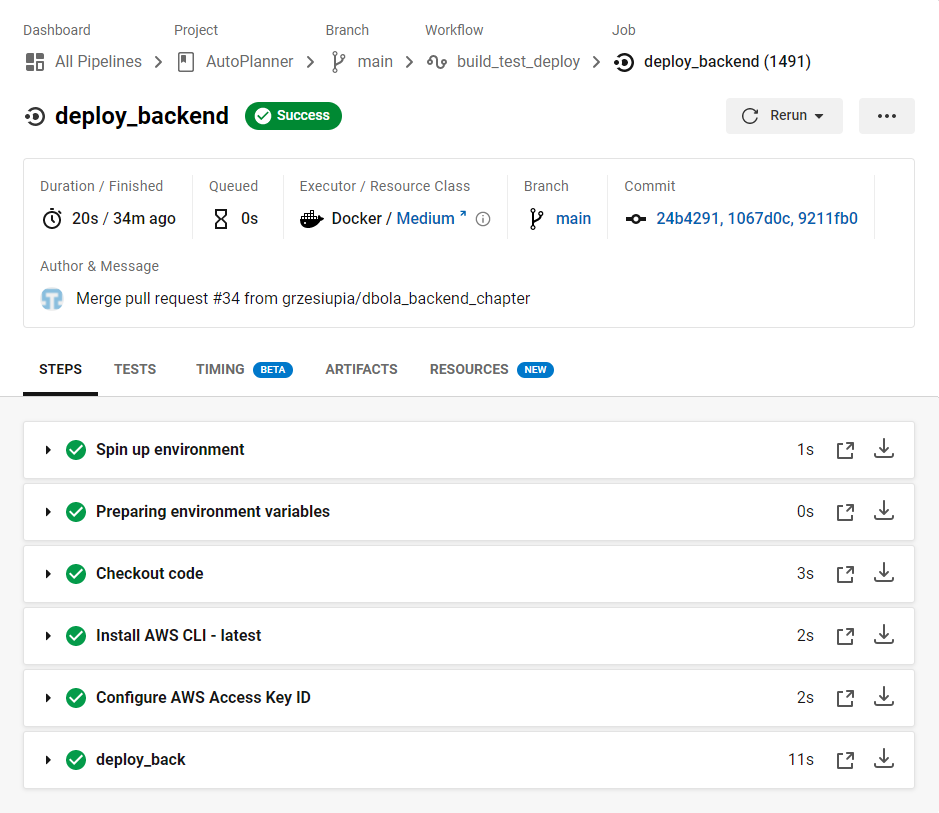
\includegraphics[width=\textwidth]{figures/circleci_deploy_back}
\caption{Przykładowy przebieg zadania \textit{deploy\_backend}. Uruchomiony dla zmian wprowadzonych w branch'y \textit{main}.}
\end{figure}
\end{itemize}

	\subsection{Zastosowanie DevOps lifecycle od strony GitHub}
	W celu zwiększenia jakości dostarczanych rozwiązań zastosowano następujący przebieg wdrażania. Członek zespołu chcąc wprowadzić nową funkcjonalność lub rozwinąć już istniejącą zaciąga najnowszą wersję projektu ze zdalnego repozytorium. Gdy lokalne repozytorium jest zaktualizowane, deweloper tworzy nową \textit{branch}, w której będzie wprowadzał zmiany. W momencie gdy autor chce podzielić się swoją pracą z innymi członkami zespołu push'uje swoje zmiany do zdalnego repozytorium oraz tworzy \textit{Pull Request} (PR). W takim PR można prześledzić wszystkie zmiany jakie zostały po kolei wprowadzone przez autora. Każda wprowadzona zmiana pojawiająca się w zdalnym repozytorium wywołuje uruchomienie pipeline'y na platformie CircleCI. Wynik działania zadań z uruchomionego workflow również można sprawdzić z poziomu PR. W przypadku gdy zmiany wprowadzone w ramach PR przechodzą wszystkie testy oraz nie wywołują żadnych konfliktów autor prosi o sprawdzenie i zatwierdzenie zmian przez innego członka zespołu. Gdy współpracownik zatwierdzi zmiany, może zostać wykonany merge do branch'y \textit{main}. Po wprowadzeniu zmian do \textit{main} następuje ostatni etap tj. uruchomienie pipeline'y z poziomu tej branch'y a co za tym idzie ponowne zbudowanie i przetestowanie aplikacji oraz ostatecznie \textit{deployment}.
\begin{figure}[H]
\centering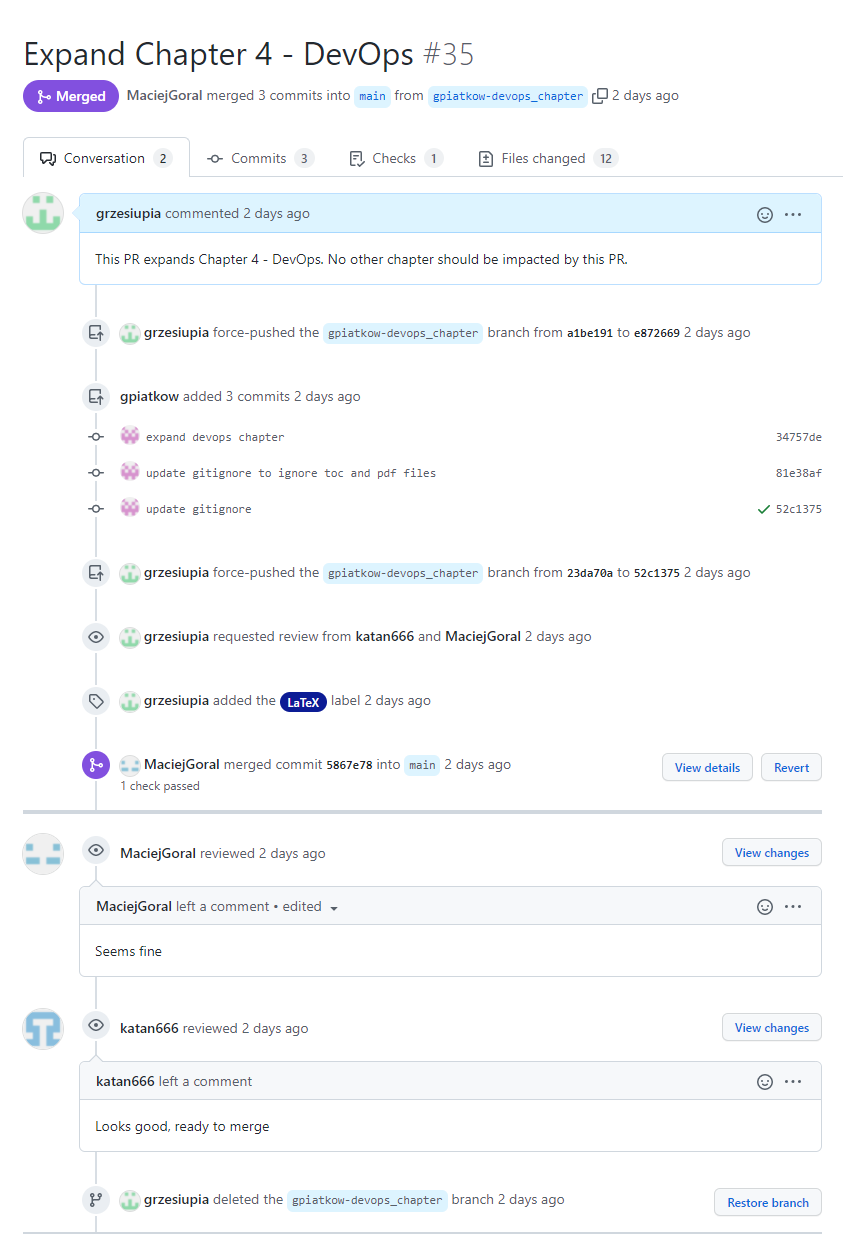
\includegraphics[width=\textwidth]{figures/github_pr}
\caption{Przykładowy przebieg wdrażania zmian przy pomocy \textit{Pull Request}}
\end{figure}
	
	 